% Options for packages loaded elsewhere
\PassOptionsToPackage{unicode}{hyperref}
\PassOptionsToPackage{hyphens}{url}
%
\documentclass[
]{article}
\usepackage{lmodern}
\usepackage{amssymb,amsmath}
\usepackage{ifxetex,ifluatex}
\ifnum 0\ifxetex 1\fi\ifluatex 1\fi=0 % if pdftex
  \usepackage[T1]{fontenc}
  \usepackage[utf8]{inputenc}
  \usepackage{textcomp} % provide euro and other symbols
\else % if luatex or xetex
  \usepackage{unicode-math}
  \defaultfontfeatures{Scale=MatchLowercase}
  \defaultfontfeatures[\rmfamily]{Ligatures=TeX,Scale=1}
\fi
% Use upquote if available, for straight quotes in verbatim environments
\IfFileExists{upquote.sty}{\usepackage{upquote}}{}
\IfFileExists{microtype.sty}{% use microtype if available
  \usepackage[]{microtype}
  \UseMicrotypeSet[protrusion]{basicmath} % disable protrusion for tt fonts
}{}
\makeatletter
\@ifundefined{KOMAClassName}{% if non-KOMA class
  \IfFileExists{parskip.sty}{%
    \usepackage{parskip}
  }{% else
    \setlength{\parindent}{0pt}
    \setlength{\parskip}{6pt plus 2pt minus 1pt}}
}{% if KOMA class
  \KOMAoptions{parskip=half}}
\makeatother
\usepackage{xcolor}
\IfFileExists{xurl.sty}{\usepackage{xurl}}{} % add URL line breaks if available
\IfFileExists{bookmark.sty}{\usepackage{bookmark}}{\usepackage{hyperref}}
\hypersetup{
  pdftitle={Which Variables help in predicting supermarket revenue? Evidence from Chicago},
  hidelinks,
  pdfcreator={LaTeX via pandoc}}
\urlstyle{same} % disable monospaced font for URLs
\usepackage[margin=1in]{geometry}
\usepackage{graphicx,grffile}
\makeatletter
\def\maxwidth{\ifdim\Gin@nat@width>\linewidth\linewidth\else\Gin@nat@width\fi}
\def\maxheight{\ifdim\Gin@nat@height>\textheight\textheight\else\Gin@nat@height\fi}
\makeatother
% Scale images if necessary, so that they will not overflow the page
% margins by default, and it is still possible to overwrite the defaults
% using explicit options in \includegraphics[width, height, ...]{}
\setkeys{Gin}{width=\maxwidth,height=\maxheight,keepaspectratio}
% Set default figure placement to htbp
\makeatletter
\def\fps@figure{htbp}
\makeatother
\setlength{\emergencystretch}{3em} % prevent overfull lines
\providecommand{\tightlist}{%
  \setlength{\itemsep}{0pt}\setlength{\parskip}{0pt}}
\setcounter{secnumdepth}{-\maxdimen} % remove section numbering

\title{Which Variables help in predicting supermarket revenue? Evidence from
Chicago}
\author{}
\date{\vspace{-2.5em}}

\begin{document}
\maketitle

\hypertarget{introduction}{%
\subsection{Introduction}\label{introduction}}

Location choice is critical to retail organization, due to its effect on
supermarket success (Clarkson, Clarke-Hill, and Robinson 1996). To
choose the outlet location, previous studies have suggested that the
location of supermarkets largely depends on the local demographic
profile (Baviera-Puig, Buitrago-Vera, and Escriba-Perez 2016). Our study
considers 45 demographic variables and tries to answer the research
question: what demographic variables are important for predicting the
revenue of supermarkets? We examine which variables have the biggest
impact through an elastic net. This model is chosen because it has shown
to work better than other regularized regressions, such as the least
absolute shrinkage method (LASSO), when several variables are highly
correlated (Zou and Hastie 2005). This is the case in our dataset. We
assess the best parameters for the model using k-fold cross validation
to further prevent overfitting (Friedman, Hastie, and Tibshirani 2001).
We find that the \% of households with children under 9 years old, \%
unemployed, and \% of households with a mortgage matter most. \#\# Data
Our research works with a dataset of 45 demographic variables related to
77 supermarkets located around the Chicago area from the year of 1996.
We define demographic data as data that reflects a profile of the
customers; examples of such data included in our data include age, sex,
income level, race, employment, homeownership, and level of education.
The variables are all continuous. A full description of each variable
included can be found in table A of the appendix, and table B includes
the summary statistics. Past studies have indicated that these variables
likely affect the supermarket turnover. For example, the variable of
income has a relation to food consumption in supermarkets (Jones 1997);
the variable of gender may influence the choice of supermarket (Beynon,
Moutinho, and Veloutsou 2010); and the variable of race composition may
have an impact on supermarket location(Lamichhane et al. 2013). Our
response variable is yearly total turnover (\$). The demographic data
were derived from the U.S. government's (1990) census for the Chicago
metropolitan area. We scale both the independent and dependent variables
as follows:\\
\begin{align*}
\mathbf{\tilde{X}} = \frac{\mathbf{X} - \mu}{\sqrt{\frac{\sum \boldsymbol{\mathbf{X}^2}}{n-1}}}
\end{align*} Where \(\tilde{X}\) is the scaled variable, \(X\) is the
unscaled variable, \(\mu\) is the mean of \(\boldsymbol{X}\), and \(n\)
denotes the sample size. This scaling is done to ensure a fair
interpretation of the model coefficients, as the range of each variable
is different. Table C of the appendix shows that several variables are
highly correlated. It is to be expected that characteristics such as
income, home ownership, age etc. are to a large extent correlated.

\hypertarget{method}{%
\subsection{Method}\label{method}}

In short, our method is using an elastic net, which deals with
overfitting by using a weighted average of the penalty terms applied in
the LASSO and ridge regression. Before we explain the elastic net, let's
consider the standard linear regression model: \begin{align*}
    \hat{\boldsymbol{y}} = \mathbf{X}\boldsymbol{\hat{\beta}}
\end{align*} In which \(\hat{\boldsymbol{y}}\) is an n x 1 column vector
of the predicted response variable, \(\mathbf{X}\) is an n x (p+1)
matrix with n observations of p predictor variables and the intercept.
\(\boldsymbol{\hat{\beta}}\) is an (1 + p) x 1 column vector of the
estimated coefficients for true parameter \(\boldsymbol{{\beta}}\) of
the intercept and \(p\) predictor variables. The standard method for
finding the optimal \(\boldsymbol{\beta}\) is the ordinary least squared
(OLS) method that minimizes the sum of squared error between the
predicted and observed response variables \(\hat{\boldsymbol{y}}\) and
\({\boldsymbol{y}}\). Thus the following loss function is minimized:
\begin{align*}
    L(\boldsymbol{\beta}) = (\boldsymbol{y} - \mathbf{X}\boldsymbol{\beta})^T(\boldsymbol{y} - \mathbf{X}\boldsymbol{\beta}).
\end{align*} The problem with using this method is that it is prone to
overfitting (Friedman, Hastie, and Tibshirani 2001). This is because
when applied to a training set, it often overestimates the effect of
certain variables. To solve this problem, regularized regression methods
can be used. These apply penalty terms to the above loss function in
order to shrink the \(\boldsymbol{\beta}\). Elastic net is a regularized
regression that combines two penalty terms: \begin{align*}
    L_1(\boldsymbol{\beta}) = \lambda \sum_{i=1}^{p} \vert \beta_i \vert \hspace{35pt} L_2(\boldsymbol{\beta}) = \lambda. \boldsymbol{\beta}^T\boldsymbol{\beta}
\end{align*} In which \(L_1, L_2\) are the two penalty terms, and
\(\lambda\) is a constant parameter that determines their size. The
\(P_1\) is the sum of the absolute value of the coefficients, and is
used in the so-called LASSO method (Tibshirani 1996). When this penalty
term is used, coefficients are continuously reduced, or removed
completely. But using just this penalty term has several downsides; it
performs less well when \(p \geq n\), and when several variables are
highly correlated (Zou and Hastie 2005) . Zhou and Hastie (2005) show
that in these circumstances, the elastic net performs better than the
Lasso, by adding a second penalty term, \(P_2\). This is the same
penalty used in a ridge regression (Hoerl and Kennard 1970). Elastic net
then determines the weight between the two penalty terms, using the
constant parameter \(\alpha\). Given the high correlation between
several of the variables in our dataset, it seems appropriate to use the
elastic net. This gives the following loss function: \begin{align*}
    L(\boldsymbol{\beta}) = (\boldsymbol{y} - \mathbf{X}\boldsymbol{\beta})^T(\boldsymbol{y} - \mathbf{X}\boldsymbol{\beta}) + \lambda \alpha \sum_{i=1}^{p} \vert \beta_i \vert + \lambda (1-\alpha) \boldsymbol{\beta}^T\boldsymbol{\beta}
\end{align*} In order to find the \(\boldsymbol{\beta}\) at which
\(L(\boldsymbol{\beta})\) is minimized, we use the majorize-minimization
algorithm (MM). We use the following majorization function:
\begin{align*}
    L(\boldsymbol{\beta})=\frac{1}{2}\boldsymbol{\beta}^T(\mathbf{A})\boldsymbol{\beta} - n^{-1}\boldsymbol{\beta}^T\mathbf{X}^T\boldsymbol{y} + c \\
\end{align*} \begin{align*}
    \mathbf{A} = n^{-1}\mathbf{X}^T\mathbf{X} + \lambda(1+\alpha)I + \lambda \alpha \mathbf{D} \hspace{35pt}
    \mathbf{D} = \begin{bmatrix}
    \frac{1}{max(\beta_1, \epsilon)} &0 &0 \\
    0& \ddots & 0\\
    0& 0& \frac{1}{max(\beta_p, \epsilon)} \\
  \end{bmatrix} \hspace{35pt}
   c = \frac{1}{2n}\boldsymbol{y}^T\boldsymbol{y} + \frac{1}{2}\lambda\alpha  \sum_{i=1}^{p} \vert \beta_i \vert
\end{align*} We then find the \(\boldsymbol{\beta}\) for which this
function is minimized through stepwise updating the
\(\boldsymbol{\beta}\). This happens by solving the following:
\(\hat{\boldsymbol{\beta_k}} = (\mathbf{A})^{-1}n^{-1}\mathbf{X}^T\boldsymbol{y}\).
Here, \(\hat{\boldsymbol{\beta_k}}\) is the estimated
\(\boldsymbol{\beta}\) at step k. This stepwise updating continues until
the next set of \(\boldsymbol{\beta}\) does not improve the loss
functionby more than \(\epsilon\). To find the \(\lambda\) and
\(\alpha\) for our elastic net, we use K-fold cross validation. In this
method, the dataset is split into \(K\) random samples. One of the
samples is picked as the validation set, and the \(\boldsymbol{\beta}\)
are determined based on the remaining K-1 samples. This then happens K
times, until each of the samples is used as a validation set. For each
iteration, we calculate the root mean squared error (RMSE), and then the
average RMSE across the K validations. \begin{align*}
    RMSE = \sqrt{ \frac{1}{n} \sum_{i=1}^{n} (\hat{\boldsymbol{y}} - \boldsymbol{y})^2 } \hspace{35pt} \text{Average RMSE} = \frac{1}{K}\sum_{i=1}^{K} RMSE_i 
\end{align*}\\
In which \(RMSE_i\) is the RMSE of the validation on sample \(i\). Our
metric for picking the \(\lambda\) and \(\alpha\) is the lowest average
RMSE. The process of finding this metric process is visualized below for
K = 4.

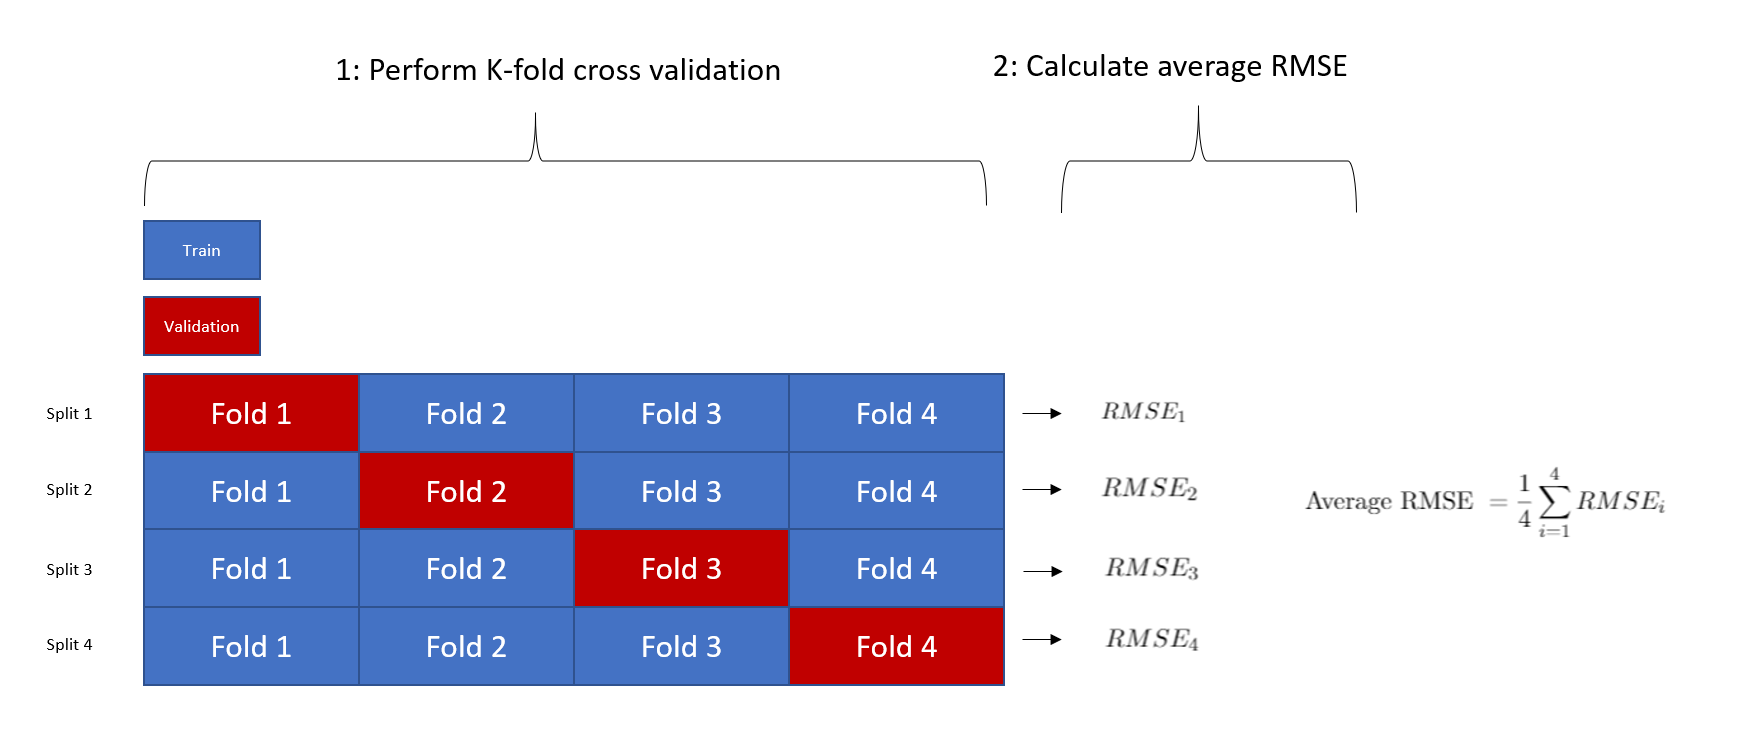
\includegraphics[]{kfold.PNG}

Using K-fold cross validation to pick the ideal \(\lambda, \alpha\)
reduces the likelihood of overfitting, since the parameters are not just
based on one random sample, but on multiple, reducing the likelihood
that features from one sample dominate when predicting. We fold our
sample 10 times - this allows us to use a lot of different folds,
without becoming computationally too expensive. We use RMSE to measure
the error between our prediction and the actual values. The squaring of
these errors ensures that larger errors contribute more to the loss
function, which decreases the chance of our model making large mistakes.
When searching for \(\lambda\), \(\alpha\), we evaluate all combinations
between two sets. The first set containing all possible \(\alpha\)
values is defined as follows: \(\alpha = \{0.1, 0.2,..., 1\}\). The set
containing the \(\lambda\) values is
\(\lambda = \{10^{x_{1}}, 10^{x_{2}},..., 10^{x_{50}}\}\) with \(x\)
increasing from \(-2\) to \(10\) in 50 steps.

\hypertarget{results}{%
\subsection{Results}\label{results}}

By minimizing the RMSE of all \(\alpha\) and \(\lambda\) combinations,
we find that an \(\alpha\) of 0.2 and \(\lambda\) of 0.1 produces the
best fitted model. This indicates that in our problem more emphasis
should be put on the \(L_2\) penalty. This result is consistent with the
findings in (Marquardt and Snee 1975), which found that in problems with
highly correlated explanatory variables ridge regression performs best.

To answer our research question on what variables are most important for
the prediction of supermarket turnover we analyse the estimated
coefficients obtained by training on the scaled dataset. These are found
in table \href{resultTable}. In this table only the coefficients with an
absolute value higher than 0.01 are displayed, because any coefficients
below this threshold are at least an order of magnitude smaller and thus
have extremely little effect on our dependent variable. The coefficients
represent change in our standardised dependent variable when the
independent variable changes with one standard deviation. Thus the
absolute size of the coefficient can be interpreted as the contribution
of the variable for the prediction. From table
\href{resultTable} we find that the three most influential variables are the $\%$ of households with children under nine years old, $\%$ unemployed and percentage of households with a mortgage. Here the first two are positive in their influence on supermarket turnover and the last one is negative.

\hypertarget{refs}{}
\leavevmode\hypertarget{ref-baviera2016geomarketing}{}%
Baviera-Puig, Amparo, Juan Buitrago-Vera, and Carmen Escriba-Perez.
2016. ``Geomarketing Models in Supermarket Location Strategies.''
\emph{Journal of Business Economics and Management} 17 (6): 1205--21.

\leavevmode\hypertarget{ref-beynon2010gender}{}%
Beynon, Malcolm J, Luiz Moutinho, and Cleopatra Veloutsou. 2010.
``Gender Differences in Supermarket Choice.'' \emph{European Journal of
Marketing}.

\leavevmode\hypertarget{ref-clarkson1996uk}{}%
Clarkson, Richard M, Colin M Clarke-Hill, and Terry Robinson. 1996. ``UK
Supermarket Location Assessment.'' \emph{International Journal of Retail
\& Distribution Management}.

\leavevmode\hypertarget{ref-friedman2001elements}{}%
Friedman, Jerome, Trevor Hastie, and Robert Tibshirani. 2001. \emph{The
Elements of Statistical Learning}. Vol. 1. 10. Springer series in
statistics New York.

\leavevmode\hypertarget{ref-hoerl1970ridge}{}%
Hoerl, Arthur E, and Robert W Kennard. 1970. ``Ridge Regression: Biased
Estimation for Nonorthogonal Problems.'' \emph{Technometrics} 12 (1):
55--67.

\leavevmode\hypertarget{ref-jones1997analysis}{}%
Jones, Eugene. 1997. ``An Analysis of Consumer Food Shopping Behavior
Using Supermarket Scanner Data: Differences by Income and Location.''
\emph{American Journal of Agricultural Economics} 79 (5): 1437--43.

\leavevmode\hypertarget{ref-lamichhane2013spatial}{}%
Lamichhane, Archana P, Joshua Warren, Robin Puett, Dwayne E Porter,
Matteo Bottai, Elizabeth J Mayer-Davis, and Angela D Liese. 2013.
``Spatial Patterning of Supermarkets and Fast Food Outlets with Respect
to Neighborhood Characteristics.'' \emph{Health \& Place} 23: 157--64.

\leavevmode\hypertarget{ref-marquardt1975ridge}{}%
Marquardt, Donald W, and Ronald D Snee. 1975. ``Ridge Regression in
Practice.'' \emph{The American Statistician} 29 (1): 3--20.

\leavevmode\hypertarget{ref-tibshirani1996regression}{}%
Tibshirani, Robert. 1996. ``Regression Shrinkage and Selection via the
Lasso.'' \emph{Journal of the Royal Statistical Society: Series B
(Methodological)} 58 (1): 267--88.

\leavevmode\hypertarget{ref-zou2005regularization}{}%
Zou, Hui, and Trevor Hastie. 2005. ``Regularization and Variable
Selection via the Elastic Net.'' \emph{Journal of the Royal Statistical
Society: Series B (Statistical Methodology)} 67 (2): 301--20.

\end{document}
